% !TeX root = document.tex
% !TeX encoding = UTF-8 Unicode

%================================================================================================
%=========================================== CAPA 1 =============================================
%================================================================================================

\vspace*{1.0cm}

\begin{center}
    {\textsc  Centro Federal de Educaçào Tecnológica de Minas Gerais\\
        \textit{Campus} Divinópolis\\
        Graduação em Engenharia Mecatrônica}
\end{center}

\vspace*{3.0cm}

\begin{center}
    \large Álan Crístoffer e Sousa
\end{center}

\vspace*{2.5cm}

\begin{center}
    \Large{\textsc{Implementação de controlador MPC em um sistema a parâmetros
                  distribuídos via subsistemas interconectados}} % alterar
                  % também mais abaixo.
\end{center}

\vspace*{4cm}

\epsfxsize=0.175\columnwidth{}
\centerline{\epsffile{imgs/cefet.eps}}

\null\vfill

\begin{center}
    Divinópolis\\
    \(2018\) % alterar também mais abaixo.
\end{center}

\thispagestyle{empty}
\cleardoublepage{}

%================================================================================================
%=========================================== CAPA 2 =============================================
%================================================================================================

\vspace*{1cm}

\begin{center}
    \large Álan Crístoffer e Sousa
\end{center}

\vspace*{1.5cm}

\begin{center}
    \Large{\textsc{Implementação de controlador MPC em um sistema a parâmetros
                  distribuídos via subsistemas interconectados}} % alterar
                  % também mais acima.
\end{center}

\vspace*{1.5cm}

\begin{flushright}
    \begin{minipage}{9.0cm}
        Monografia de Trabalho de Conclusão de Curso apresentada ao Colegiado de
        Graduação em Engenharia Mecatrônica como  parte dos requisitos exigidos
        para a obtenção do título de Engenhario Mecatrônico.\\
        Eixo de Formação: Modelagem e Controle de Processos.

        \vspace*{1cm}

        Orientador: Prof.\ Dr.\ Valter Júnior de Souza Leite\\
        Coorientador: Prof.\ Dr.\ Ignacio Rubio Scola
    \end{minipage}
\end{flushright}

\vspace*{1cm}

\epsfxsize=0.175\columnwidth{}
\centerline{\epsffile{imgs/cefet.eps}} % Aqui poderia ser substituido por um logo do curso ou do campus

\null\vfill

\begin{center}
    Divinópolis\\
    \(2018\) % alterar também mais acima.
\end{center}

\cleardoublepage{}

%================================================================================================
%============================== Ficha (Somente na versão final) =================================
%================================================================================================

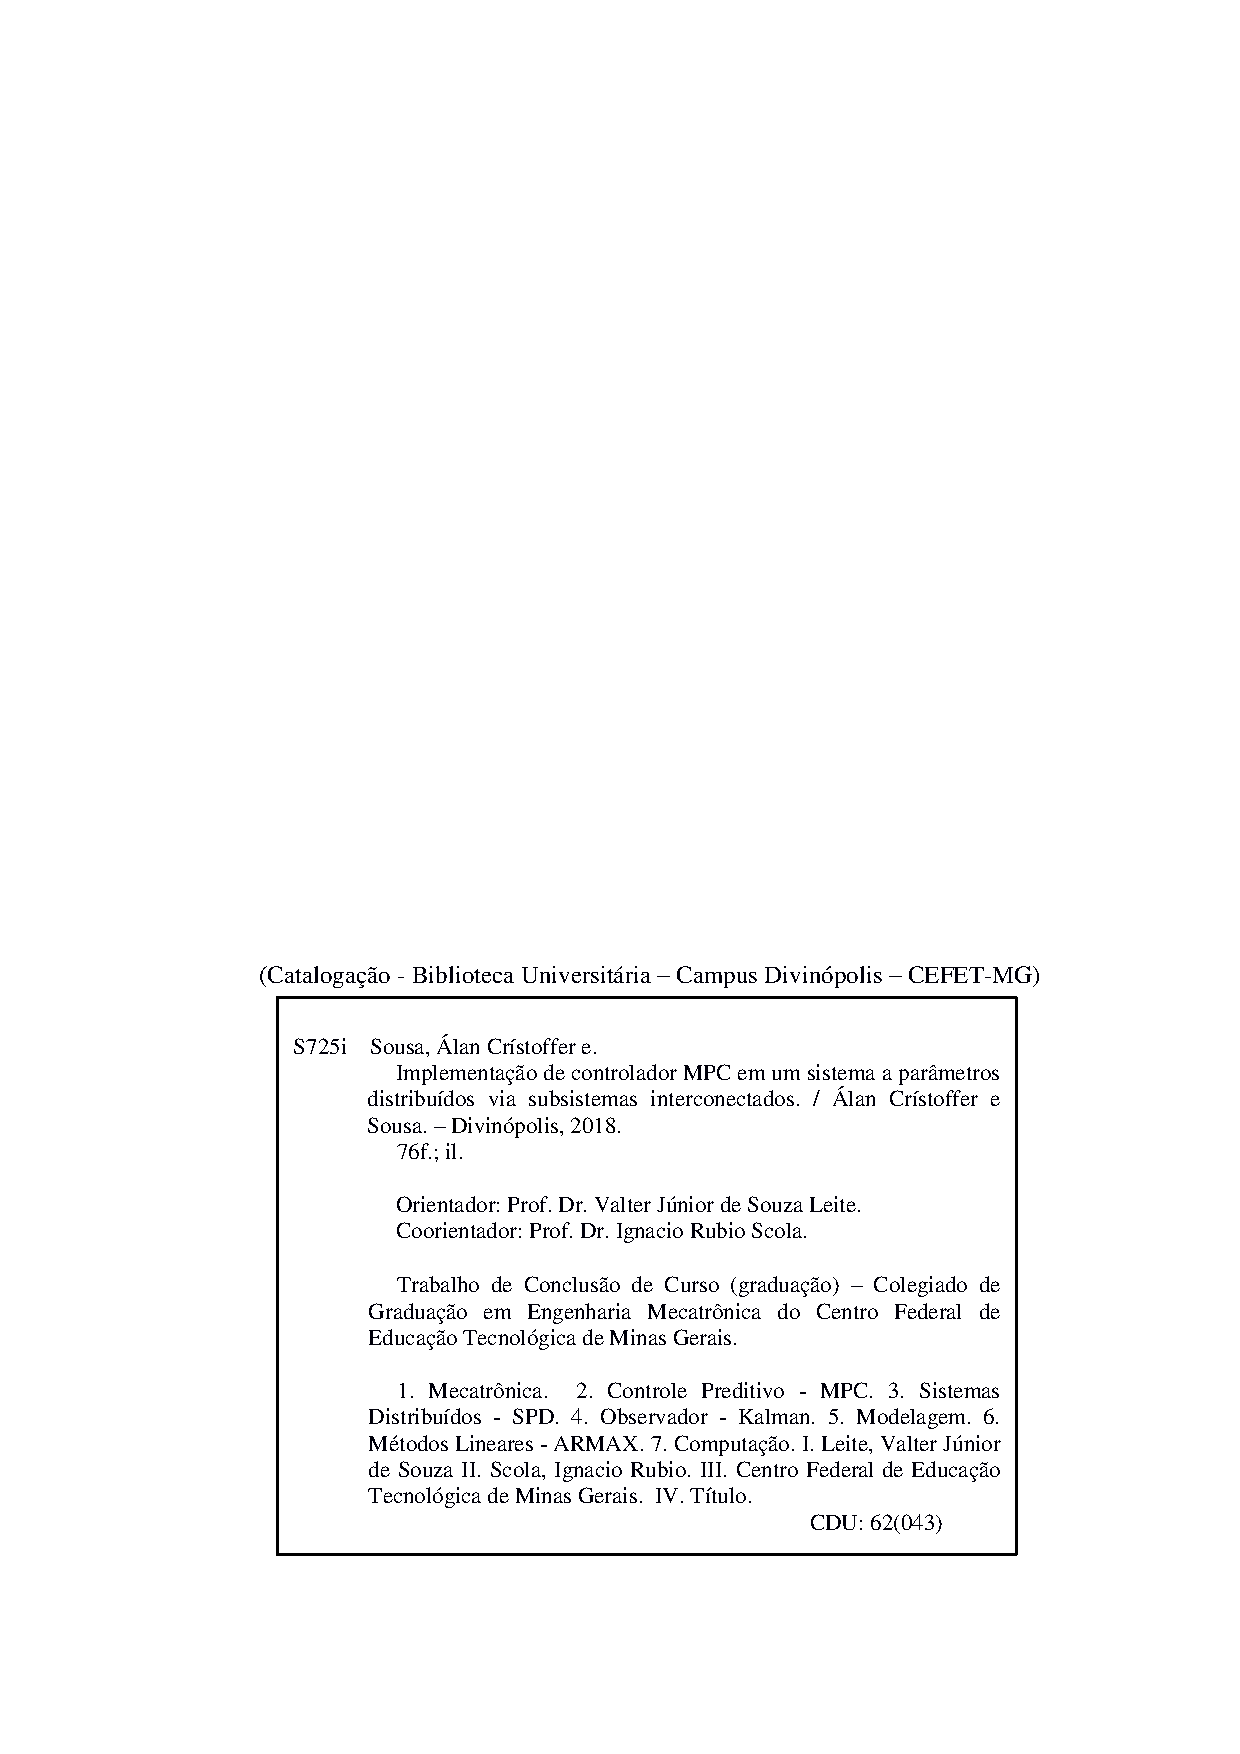
\includepdf[pages=-]{ficha.pdf} % após scanear, colocar a ficha catalográfica do texto
\cleardoublepage{}

%================================================================================================
%============================== Folha de aprovação (Somente na versão final) ====================
%================================================================================================

\begin{table}[]
    \begin{tabular}{ll}
    \multirow{3}{*}{\includegraphics[width=3cm]{imgs/cefet}} & Centro Federal de Educação Tecnológica de Minas Gerais \\
                                                             & CEFET-MG / Divinópolis                                 \\
                                                             & Curso de Engenharia Mecatrônica                       
    \end{tabular}
\end{table}

\vspace*{2.0cm}

Monografia entitulada \enquote{Implementação de controlador MPC em um sistema
a parâmetros distribuídos via subsistemas interconectados}, de autoria do
graduando Álan Crístoffer e Sousa, aprovada pela banca examinadora constituída
pelos seguintes professores:

\vspace*{1cm}

\begin{center}
    \hrulefill{}\\
    Prof.\ Dr.\ Valter Júnior de Souza Leite

    \vspace*{1cm}

    \hrulefill{}\\
    Prof.\ Me.\ Alberto Pena Lara

    \vspace*{1cm}

    \hrulefill{}\\
    Prof.\ Me.\ Adriano Nogueira Drumond Lopes

    \vspace*{4cm}

    \hrulefill{}\\
    Coordenador do Curso de Engenharia Mecatrônica\\
    Prof.\ Dr.\ Lúcio Flávio Santos Patrício\\
~\\
    Divinópolis\\
    Dezembro de 2018
\end{center}

\vfill{}
\cleardoublepage{}
